% THIS IS SIGPROC-SP.TEX - VERSION 3.1
% WORKS WITH V3.2SP OF ACM_PROC_ARTICLE-SP.CLS
% APRIL 2009
%
% It is an example file showing how to use the 'acm_proc_article-sp.cls' V3.2SP
% LaTeX2e document class file for Conference Proceedings submissions.
% ----------------------------------------------------------------------------------------------------------------
% This .tex file (and associated .cls V3.2SP) *DOES NOT* produce:
%       1) The Permission Statement
%       2) The Conference (location) Info information
%       3) The Copyright Line with ACM data
%       4) Page numbering
% ---------------------------------------------------------------------------------------------------------------
% It is an example which *does* use the .bib file (from which the .bbl file
% is produced).
% REMEMBER HOWEVER: After having produced the .bbl file,
% and prior to final submission,
% you need to 'insert'  your .bbl file into your source .tex file so as to provide
% ONE 'self-contained' source file.
%
% Questions regarding SIGS should be sent to
% Adrienne Griscti ---> griscti@acm.org
%
% Questions/suggestions regarding the guidelines, .tex and .cls files, etc. to
% Gerald Murray ---> murray@hq.acm.org
%
% For tracking purposes - this is V3.1SP - APRIL 2009

\documentclass{acm_proc_article-sp}

\newdef{definition}{Definition}

\makeatletter
\newif\if@restonecol
\makeatother
\let\algorithm\relax
\let\endalgorithm\relax
\usepackage[ruled,vlined]{algorithm2e}

\usepackage{enumerate}


\begin{document}

\title{EasyMerge - A New Tool for Code Clones Refactoring}
%
% You need the command \numberofauthors to handle the 'placement
% and alignment' of the authors beneath the title.
%
% For aesthetic reasons, we recommend 'three authors at a time'
% i.e. three 'name/affiliation blocks' be placed beneath the title.
%
% NOTE: You are NOT restricted in how many 'rows' of
% "name/affiliations" may appear. We just ask that you restrict
% the number of 'columns' to three.
%
% Because of the available 'opening page real-estate'
% we ask you to refrain from putting more than six authors
% (two rows with three columns) beneath the article title.
% More than six makes the first-page appear very cluttered indeed.
%
% Use the \alignauthor commands to handle the names
% and affiliations for an 'aesthetic maximum' of six authors.
% Add names, affiliations, addresses for
% the seventh etc. author(s) as the argument for the
% \additionalauthors command.
% These 'additional authors' will be output/set for you
% without further effort on your part as the last section in
% the body of your article BEFORE References or any Appendices.

\numberofauthors{3} %  in this sample file, there are a *total*
% of EIGHT authors. SIX appear on the 'first-page' (for formatting
% reasons) and the remaining two appear in the \additionalauthors section.
%
\author{
% You can go ahead and credit any number of authors here,
% e.g. one 'row of three' or two rows (consisting of one row of three
% and a second row of one, two or three).
%
% The command \alignauthor (no curly braces needed) should
% precede each author name, affiliation/snail-mail address and
% e-mail address. Additionally, tag each line of
% affiliation/address with \affaddr, and tag the
% e-mail address with \email.
%
% 1st. author
\alignauthor
Shengying Pan\\
       \affaddr{School of Computer Science}\\
       \affaddr{University of Waterloo}\\
       \email{s5pan@uwaterloo.ca}
% 2nd. author
\alignauthor
Haocheng Qin\\
       \affaddr{School of Computer Science}\\
       \affaddr{University of Waterloo}\\
       \email{h7qin@uwaterloo.ca}
% 3rd. author
\alignauthor Yahui Chen\\
       \affaddr{School of Computer Science}\\
       \affaddr{University of Waterloo}\\
       \email{y556chen@uwaterloo.ca}
\and  % use '\and' if you need 'another row' of author names
}
% There's nothing stopping you putting the seventh, eighth, etc.
% author on the opening page (as the 'third row') but we ask,
% for aesthetic reasons that you place these 'additional authors'
% in the \additional authors block, viz.
\additionalauthors{Additional authors: John Smith (The Th{\o}rv{\"a}ld Group,
email: {\texttt{jsmith@affiliation.org}}) and Julius P.~Kumquat
(The Kumquat Consortium, email: {\texttt{jpkumquat@consortium.net}}).}
\date{30 July 1999}
% Just remember to make sure that the TOTAL number of authors
% is the number that will appear on the first page PLUS the
% number that will appear in the \additionalauthors section.

\maketitle
\begin{abstract}
Code clones are common in medium to large scale software projects. Oftentimes, unnecessary clones cause troubles to code base maintenance and code reusability. 
Over past decades, many techniques and approaches have been proposed to detect code clones. However, how to refactor clones is still a very challenging topic to software
engineers. Even text-wise identical code clones can be semantically different when they are referring variables and calling functions outside. And the problem is more 
complex when scopes and dependencies are involved. Furthermore, not all clones shall be refactored as they may be part of independent
libraries. And refactoring is not only about removing duplicate code but also fixing all reference errors caused by such deletion thereafter. 
As a result, we need adaptive clone refactoring tools that can locate unnecessary clones and alert possible implications in the procedure to help
software engineers be more efficient and make less mistakes in the refactoring process.

In this paper, we introduce EasyMerge, a new tool to refactor code clones. EasyMerge is built on top of AST-based anti-unification clone detection algorithm and 
refactors software projects written in Python. It adds intelligence to code clone refactoring by categorizing clones and generating refactoring recommendations
based on evaluation of external variable references and function calls. It copes with features of Python language and can deal with clone fragments across different scopes. 
It ensures functionality-wise consistency before and after refactoring and provide warnings when potential refactoring could lead to
unwanted complexity or cause readability issues.
\end{abstract}

% A category with the (minimum) three required fields
%\category{H.4}{Information Systems Applications}{Miscellaneous}
%A category including the fourth, optional field follows...
\category{D.2.7}{Software Engineering}{Maintenance}[Restructuring, reverse engineering, and reengineering]

\terms{Algorithms}

\keywords{Software engineering, clone detection, code refactoring, recommendation system, Python} % NOT required for Proceedings

\section{Introduction}
In software development, it's very common seeing developers reuse code fragments by copying and pasting with or without minor adaptation.
Moreover, for large scale projects, developers are often too lazy to browse existing source files so that they may rewrite similar or even identical functions which
were already in the code base. As a result, software systems often contain sections of code that are very similar, called code clones.

Previous research shows that a significant fraction (between 7\% and 23\%) of the code in a typical software system has been cloned \cite{baker} \cite{roy1}. Many code clones
in code bases are unnecessary duplications. 
Code duplication can be a significant drawback, leading to bad design, and increased probability of bug occurrence and propagation. As a result, it can significantly
increase maintenance cost, and form a barrier for software evolution. By detecting, categorizing,
and removing code clones, we can produce easier to understand, cleaner, and more reusable code.

Clone detection has been an avid research topic in the field of software engineering for decades. Fortunately, several automated techniques for detecting code clones
have already been proposed. However, how to deal with detected clones, e.g. how to distinguish necessary clones from unnecessary ones and how to refactor code to remove
unnecessary clones still remain a big problem in not only commercial but also academic domain. In this paper, we try to classify code clones and build
a recommendation system called EasyMerge to help developers merge unnecessary clones on top of current state-of-the-art clone detection approach.

More specifically, we pick CloneDigger \cite{bulychev}, an anti-unification duplicate code detection tool as our underlying clone detector. CloneDigger is one of the best available 
clone detection tools for its overall performance, coverage of multiple clone types, and availability. 
EasyMerge integrates CloneDigger as the pre-processing tool, analyze its output clone pairs, and recommend possible merges which can remove unnecessary clones without changing functionality of code base, creating reference conflicts, nor causing troubles to future code understanding and reusing.

The rest of the paper is structured as follows: we first go through the basics, background, and current state of clone detection and code clone refactoring in general.
Then we introduce and discuss the fundamentals of CloneDigger and the anti-unification algorithm it is using to detect clones. Afterwards, we explain EasyMerge's
work flow and underlying techniques. And at the end, we set up testing environment and discuss the experimental results of running EasyMerge against several
open source projects of different scales.

\section{Background}
\subsection{Clone Detection}
Roy, Cordy, and Koschke have done a great work \cite{roy2} writing an overview paper explaining the basics of clone detection, and providing a complete comparison of essential
strengths and weaknesses of both individual tools and techniques and alternative approaches in general. It gives us all the needed preliminaries to focus on clone refactoring rather
than spending time working on the detection part. We begin with a basic introduction to clone detection terminology in Roy's paper.

\begin{definition}
(Code Fragment). A code fragment (CF) is any sequence of code lines (with or without comments). It can be of any granularity, e.g., function
definition, begin-end block, or sequence of statements. A $CF$ is identified by its file name and begin-end line numbers in the original code base
and is denoted as a triple ($CF.FileName$, $CF.BeginLine$, $CF.EndLine$).
\end{definition}

\begin{definition}
(Code Clone). A code fragment $CF2$ is a clone of another code fragment $CF1$ if they are similar by some given definition of similarity, that is, 
$f(CF1) = f(CF2)$ where $f$ is the similarity function (see clone types below). Two fragments that are similar to each other form a clone pair
$(CF1, CF2)$, and when many fragments are similar, they form a clone class or clone group.
\end{definition}

\begin{definition}
(Clone Types). There are two main kinds of similarity between code fragments. Fragments can be similar based on the similarity of their program text,
or they can be similar based on their functionality (independent of their text). The first kind of clone is often the result of copying a code fragment and
pasting into another location. In the following we provide the types of clones based on both the textual (Type 1 to 3)\cite{bellon} and functional (Type 4)\cite{gabel, komondoor} similarities:

\begin{itemize}
\item {\bf Type-1:} Identical code fragments except for variations in whitespace, layout and comments.
\item {\bf Type-2:} Syntactically identical fragments except for variations in identifiers, literals, types, whitespace, layout and comments.
\item {\bf Type-3:} Copied fragments with further modifications such as changed, added or removed statements, in addition to variations in identifiers, literals, types, whitespace, layout and comments.
\item {\bf Type-4:} Two or more code fragments that perform the same computation but are implemented by different syntactic variants.
\end{itemize}
\end{definition}

There are many different techniques to detect code clones. In Roy's paper \cite{roy2}, they covered tools of textual approaches, lexical approaches, syntactic approaches,
semantic approaches and hybrids. Different tools have advantages and disadvantages for different facets (usage, interaction, language, clone information, technical aspect, 
adjustment, processing, and evaluation) and behave quite differently for some scenarios. As clone detection is still an on-going research, it's hard to say one tool is the best
at the moment. However, for the purpose of building EasyMerge, we want to pick a tool that is cross-platform, freely available, efficient, covering multiple clone types, and can
handle different editing scenarios decently. Thus we chose CloneDigger \cite{bulychev} after a comprehensive comparison.

\subsection{Clone Refactoring}
On the other hand, for clone refactoring, most proposed solutions use pre-defined metrics as the refactoring guidance to help users determine whether the 
code clones are suitable for refactoring. For example, Balazinska \cite{balazinska} proposed to use 21 metrics to measure the suitability for refactoring. Higo \cite{higo}
developed ARIES tools, using the code detection tool CCFinder and environment analysis tool Gemini to find the clones can be refactored. And Schulze \cite{schulze}
proposed a new metric DIST (distance of the code clones). 
%Unlike them, instead of calculating distance between code fragments and only merging close clones, EasyMerge 
%try to fix the differences and merge as many clones as possible without introducing extra complexity.

For the actual merging process, currently existing research mainly focus on using refactoring patterns \cite{fowler}, especially ``Extract Method" and ``Pull Up Method".
"Extract Method" means that a fragment of source code is extracted and redefined as a new method. ``Pull Up Method" means that the same methods defined in child
classes are pulled up to its parent class. In general, they are both merging similar code blocks into one newly created function, and ``Pull Up Method" only differs from 
``Extract Method" as it places the newly created function into the super class when code blocks are inside functions sharing the same parent class.

Unfortunately, code clones may be coupled with surrounding code, its inheritance tree, or other independent classes/code blocks. For instance, code fragments inside clone pairs
may contain function calls or variable references which are not defined inside the fragments. Furthermore, functions and variables of the same names may be in fact different
at different locations of the code base. For example, if we have a code clone fragment of following:

\IncMargin{1em}
\begin{algorithm}
	for x in range(0, 3):
	
		\Indp a = x + 1
		
		b = f(x)
		
		c = d + x
\end{algorithm}
\DecMargin{1em}

We are calling function {\bf f()} where the definition of {\bf f()} can be different from fragment to fragment. Moreover, the value of variable {\bf d} is potentially different, too.
The current approach to solve this problem is to pass such external functions and variables as parameters to newly generated methods from the ``Extract Method" refactoring pattern.
For instance:

\IncMargin{1em}
\begin{algorithm}
	def helper(p1, p2):
	
		\Indp for x in range(0, 3):
		
			\Indp a = x + 1
			
			b = p1(x)
			
			c = p2 + x
			
		\Indm \Indm helper(f, d)
	
\end{algorithm}
\DecMargin{1em}

However, this creates two new problems. Firstly, in this example, the scope of b was changed. It is now inside the helper function and no longer available to code after the clone fragment
which could potentially cause reference errors. Secondly, when the length of the clone fragment is too long, we could possibly end up with a helper function of tons of parameters
which in turn make the code after refactoring harder to understand and is against our goal to improve readability. 
For most clone refactoring approaches, this gives bad scores to the evaluation metrics and prevent merging. And a possible alternative approach
is to return b and such variables from the ``Extracted Method" which introduces even more complexity.

For recently proposed refactoring approach \cite{li} and the tools mentioned at the beginning of this subsection, they count the number of such external references
in a code clone fragment as the key factor of their refactoring guideline metrics. 
And clone fragments of too many such occurrences will not be recommended for refactoring.
Furthermore, in Li's work \cite{li}, after standardization, it can also be used to refactor some semantical
similar but syntax-wise different clones by moving different function references to extracted method's parameters.

Additionally, results from clone detectors are usually clone pairs but it's very common 
more than two fragments are clones of each other. Moreover, overlapping clone fragments often
exist in large scale code bases, too. For example, it's not difficult to find a code block of ABCDEF where BC is a clone fragment of one other block and CDE is a clone fragment of another. For both cases, merging one set of clones will in turn break clones in another set. 
And we need to take care of all reference errors caused by code deletion. 
Thus, our clone refactoring tool must handle all these potential issues without
introducing too much computational overhead.

Unlike most of current clone refactoring approaches that use token-based CCFinder \cite{kamiya} for clone detection, EasyMerge uses a newer detection tool called CloneDigger.
Compared to CCFinder, CloneDigger is cross-platform and freely available as an open source project. Moreover, based on evaluation from Roy \cite{roy2},
CloneDigger performs no worse than CCFinder in all detection scenarios and is actually better in certain scenarios e.g. a programmer copies a function that calculates the sum
and product of a loop variable and calls another function, foo() with these values as parameters three times, making changes in whitespace in the first fragment (S1(a)), changes
in commenting in the second (S1(b)), and changes in formatting in the third (S1(c)). In the following section, we will go over the basic ideas behind CloneDigger and its anti-unification
algorithm.

\section{CloneDigger}
CloneDigger \cite{bulychev} was an anti-unification code clone detector introduced by Bulychev and Minea in 2008. It's one of the latest open source clone detection tool.

\subsection{Overview}
Techniques for detecting duplicate code can be classified according to several criteria. Code can be viewed as similar based on syntactic criteria or at a semantic level. CloneDigger considers only syntactic similarity. The algorithm is approached based on abstract syntax trees. The algorithm of finding duplicates consists of several phases. In the beginning all statements are partitioned into clusters using anti-unification distance and the code is abstractly viewed as sequence of cluster identifiers. All pairs of identical sequences of cluster IDs, which have similar statements in corresponding positions, are globally checked for similarity using anti-unification distance.


\subsection{Preliminaries}
Anti-unification is a general expression of two given terms. Let $E_{1}$ and $E_{2}$ be two terms. Anti-unification E is a generalization of $E_{1}$ and $E_{2}$ if there exist two substitutions $\sigma_{1}$ and $\sigma_{2}$ such that $\sigma_{1}(E)=E_{1}$ and $\sigma_{2}(E)=E_{2}$. The most specific generalization of $E_{1}$ and $E_{2}$. The most specific generalization of $E_{1}$ and $E_{2}$ is called anti-unifier. The anti-unifier tree of two trees $T_{1}$ and $T_{2}$ is obtained by replacing some subtrees in $T_{1}$ and $T_{2}$ by special nodes.m containing term placeholders which are marked with integers, such as $?_{n}$. An anti-unifier stores only the common top-level tree structure and therefore details may be ignored.

The anti-unification distance is defined as follows: let U be the anti-unifier of two trees $T_{1}$ and $T_{2}$ with substitutions $\sigma_{1}$ and $\sigma_{2}$. $\sigma_{1}$ and $\sigma_{2}$ are mappings from the set \{$?_{1}$, $?_{2}$, ..., $?_{n}$\} to substituting trees. Anti-unification distance between $T_{1}$ and $T_{2}$ as a sum of sizes of substituting trees in $\sigma_{1}$ and $\sigma_{2}$. The distance doesn't allow the permutation of siblings or changing the number of child nodes.

\begin{figure*}
\centering
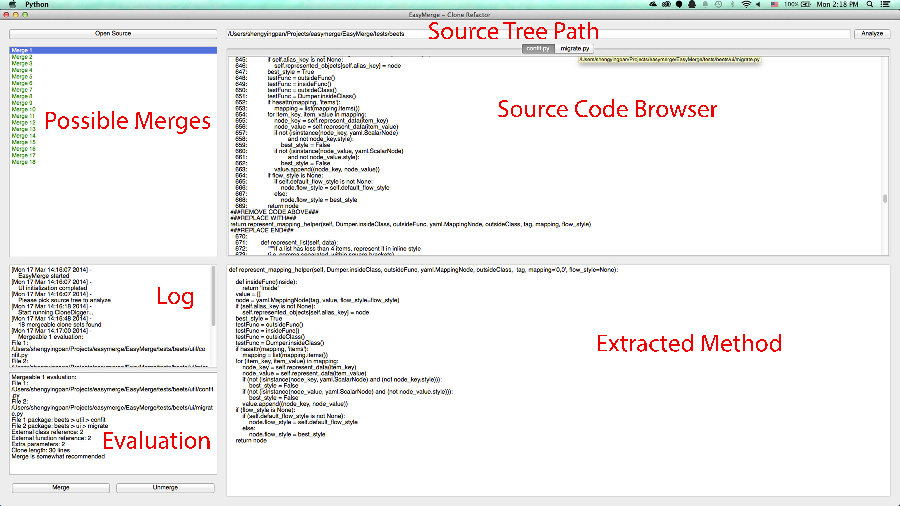
\epsfig{file=screen.pdf}
\caption{EasyMerge User Interface}
\end{figure*}

\subsection{Duplicate Code Detection Algorithm}
The method of finding duplicate code consists of three phases:
\begin{enumerate}[step 1]

    \item Partitioning similar statements into clusters
    
    Identify similar statements using anti-unification and partition them into clusters. A two-pass clustering algorithm is used. The first pass of the algorithm compare each new statement with the anti-unifiers of all existing clusters. The function $add\_cost$ is used to compute the cost of adding a tree $T$ to the cluster consisting of $n$ trees with anti-unifier $au$. Let $au'$ be the result of anti-unification of $T$ and $au$ with substitutions $\sigma_{1}$ and $\sigma_{2}$: $\sigma_{1}(au') = au$, $\sigma_{2}(au') = T$. $add\_cost$ is defined as $n \times |\sigma_{1}| + |\sigma_{2}|$. During the second pass all the statements re traversed again and for each statement we search for the most similar pattern from the set produced in the previous pass using the anti-unification distance. After the first phase each statement is marked with its cluster ID, two statements with the same cluster ID are considered similar in this preliminary view.

    \item Finding pairs of identical cluster sequences
    All pairs of sequences of statements, which are large enough, are identically labeled.
    
    \item Examining code sequences for overall similarity
    All candidates are checked as a whole using anti-unification distance. The occurrences of the same variable refers to one leaf in the abstract syntax tree increase the quality of the algorithm.
\end{enumerate}

Now we can move on to introduce EasyMerge and how it works behind the scene.


\section{EasyMerge}
The entire EasyMerge program is written with Python 2.7.5 and the user interface is powered by PyQt 4.10.4.
It takes a folder of Python written source tree as input, look for all refactorable clones and recommend potential merges.  

\subsection{User Interface}
EasyMerge has a simple and straightforward user interface, as shown in {\bf Figure 1}.
Once the program is launched, user can click ``Open Source" at top left and then choose the folder 
where the software project's source tree resides in the popup open directory dialog.
Then by clicking ``Analyze" button on the right side, EasyMerge starts analyzing the selected source tree.

There are five window boxes displayed on the main interface.
Once the scanning phase is completed, a list of refactorable clone sets are displayed in the ``Possible Merges" box at top left.
All items in the list are initially coloured green, once a merge is done, the colour will be changed to red for the record. Moreover,
the items in the list are ranked based on our recommendation evaluation from high to low.

User can click each item in the ``Possible Merges" list. When one item is selected, a corresponding clone set will be loaded. All files
associated with the set are displayed in ``Source Code Browser" tabs on the right side of the UI, where we can navigate to the
corresponding source file by clicking each tab.
Inside the source code browser, code that will be removed after merging is between ``\#\#\#REMOVE\_CODE\_BELOW\#\#\#"
and ``\#\#\#REMOVE\_CODE\_ABOVE\#\#\#". And the replacement code is between ``\#\#\#REPLACE\_WITH\#\#\#"
and ``\#\#\#REPLACE\_END\#\#\#".

On the bottom part of the screen, the ``Log" and ``Evaluation" windows are placed on the left. The ``Log" window keeps track of
program running and debugging information. Moreover, its content will also be dumped to ``log.txt" file in EasyMerge's main folder for
book keeping purpose and developers may use it to help with writing change log. The ``Evaluation" window displays evaluation metrics
for each code clone set, and will tell user whether we recommend a code merge for the set or not.

Last but not least, the ``Extracted Method" box display the extracted method we generated as a helper function all code replacement 
in original source code files are calling. After reviewing all information and recommendation we provide, a user can perform the code refactoring for
a certain set by clicking ``Merge" button on bottom left. 
EasyMerge in turn will rewrite the source files and move the generated helper to our specific accessible file in back-end.
And all merging done in current session can be redone by clicking ``Unmerge" button if
the user performed an unwanted merge for a certain set.

\subsection{Preprocessing}
The first step of EasyMerge is to run CloneDigger at target source tree, take its output and format and standardize it for our own usage.
The core of this step is to classify code clones and get the ones that we not only can but also want to merge. Although CloneDigger takes
a dozen configuration parameters, we use most of them as defaults. For our preprocessing, we only override {\bf distance-threshold} and {\bf size-threshold}
to {\bf 10} and {\bf 4} for we are only interested in clone segments of no more than 10 anti-unification distance from each other and no less than 4 lines in length.
On top of that, distance must be no more than code length as we don't want more than one difference at a line of code.

Secondly, we strip off non logical but required lines such as imports and definitions. For a code block of statements, if the last line is only a returning clause, we
modify the clone fragment by removing the returning line and keeping the rest. After text-based manipulation, we cluster all clone pairs and put them into sets
based on similarity. For example, if we have three pairs of [A, B], [B, C], [C, A] from CloneDigger's output, we generate a clone set
of [A, B, C] instead for our following merging stage.

Next, we look for overlapping code fragments in clones, to make our lives easier, for each set of overlapping clones, we only keep the longer part of the overlapping fragments
and ignore the shorter ones. For a code fragment of ABCDEFG where each letter is of the same code length, if BCD and CDEF are both duplicate code in different sets,
as they are overlapping each other,
we remove the set containing BCD and only try to merge the set with CDEF.

Additionally, if we have a set containing clone fragments which consist of both statements and function definitions, we separate and break them into multiple individual sets and guarantee that for any clone set, it either only have duplicated statements or function definition, as it's very difficult to merge multi-purpose code blocks.
For example, if we have a set of clone fragments of AFB where block A and B are statements only and F is a function definition, we will break it into three sets which
contain only A, F, and B accordingly.

Note: if you have files in the source tree that you do not want to perform analysis or merge of any kind, you need to manually exclude them from the selected folder.

\subsection{Clone Classification}
After preprocessing, we classify clone sets into multiple types as we are handling each type independently in the merging process. Firstly,
we call the anti-unifier in CloneDigger to obtain the anti-unification distance between code fragments in each clone set to determine if they
are Type-1 or Type-2 clones. Then, we check if the clone fragments in one set are in the same Python file or scattered across multiple files (this is the most common case).
Moreover, we separate duplicated functions and statements in this step as they are handled differently when extracting methods in the merging phase.

\subsection{Merging}
We first prepare merging by examine the Abstract Syntax Tree(AST) for each code clone fragment to extract some deeper information: (1) all ``import" information
(2) all class definitions and their associated scopes (3) all function calls and the scopes these calls reside. 

Then we deal with statement clones and function clones separately. For functions, we create a helper function with all code extracted from the function body.
Then we scan the code base and locate all reference calls to the original functions in the clone set and replace them with calls to the newly generated helper function.
For blocks containing only statements, similarly, we extract the code and create a helper function to host the code. And the original code blocks are replaced by
function calls to the newly generated helper function. If the clones in a set are all from the same file, we place the helper function to the same file. If they are 
from different files, we parse package dependency and find the last shared package and put the helper function there to make sure scopes are maintained properly.
Moreover, we ensure unique function name will be provided for helper functions and user can also override it in EasyMerge.

For the actual merging phase and the generation of the helper functions, 
we start with creating a potential helper function copy for each fragment in a clone set. 
We first scan for all variables, function calls and objects. Then we try to match them in 
deeper information collected before. For lines containing items that can be used without external reference, we move them directly to the copy. For everything else,
we put them into a function signature line as input parameters so we are able to use them in the future function body. 
We then look for variables and objects references to items in the 
source files happen after the clone fragment in the same scope. For any occurrence of such items, we add them to a returning line so they can still be referred to 
later in the original source files. Then we append the signature line and returning line to the helper function copy.

Last but not least, we compare each newly generated helper function copy from each fragment, if they are all identical, we use one copy as the actual extracted helper function
and write the changes to files. If not, we check if they are Type-1 clones. For Type-1 clones, we merge their individual signature line and returning line and
replace the corresponding line in the helper function copy before creating the real helper function. For non Type-1 clones, if the differences are only about constants,
we merge by replacing all constants with variables and pass them as input parameters in helper function's signature and update calls to the helper function in code base accordingly.
For other non Type-1 clones, we perform an AST pattern matching and analyzing their
symbol table and try to merge clones have same pattern of variable/function call/object referencing sequence. For a clone set of two fragments, if they both access variables
with similar patterns of a, b, a, c and e, f, e, g, then we can group [a, e], [b, f], [c, g] and treat them as three special variables in the generated helper and update
the function signature and returning line accordingly. In contrast, patterns of a, b, a, c and a, b, b, d cannot be merged. And we ignore all other clones not covered above
as they cannot be handled by EasyMerge yet.



\subsection{Recommendation Evaluation}
Although EasyMerge can handle multiple types of code clones, not all of them shall be recommended. As a matter of fact, we use a combination of 
package path analyzer and weighted evaluation formula to make our recommendation decisions. Generally speaking, we may not want to merge code
in separate libraries/packages so that we do not introduce extra coupling and each library may be used independently. 
Moreover, too many external references that pass parameters around may also be misleading and against our will to simplify code bases.
As a result, the recommendation evaluation formula is defined as following:
\begin{displaymath}
f(RE) = w_{1} * l - w_{2} * e - w_{3} * r - w_{4} * d
\end{displaymath}
where $w_{1}$, $w_{2}$, $w_{3}$, $w_{4}$ are weights,  $l$ is the number of duplicate lines, $e$ is number of external reference (including variables, functions, and objects),
$r$ is number of packed extra return values. Additionally, $d$ is the package difference defined as the the minimum package difference length in a clone set.
For example, if we have a set of two files a.b.c and a.b.d.e, the package difference length is 1 and 2 respectively as they differ after package b. And thus the $d$ value is
$min(1, 2) = 1$.

For now, we did some testing and are setting the weights at 
$w_{1} = 0.5$, $w_{2} = 1$, $w_{3} = 2$, $w_{4} = 2$ as we don't want too much externality with too few lines of code. And extra return values are more confusing than
extra input parameters. To help user make the decision, we recommend a merge if $f(RE) > 8$, somewhat recommend a merge if $ 0 \le f(RE) \le 8$, and let user merge
with cautions when $f(RE) < 0$.
It give us modest reasonable behaviour we want after some manual analysis of each clone set.
In the future, we are interested to perform a actual survey with real software developers to reconfigure these weights to better fit our purpose.



\section{Experimental Results}
All experiments are done on a desktop computer. The testing machine has an AMD FX 3.5GHz 6 cores CPU, 16 GB of memory,
128 KB L1 cache, 6 MB L2 cache (1 MB per core), and 8 MB shared L3 cache. The machine runs Ubuntu Desktop 12.04, Python
2.7.5 and has all related packages installed.
For test cases, we have two sets of open source projects written in Python. The first set contains 5 most famous projects on GitHub:
\begin{itemize}
\item Tornado - A Python web framework and asynchronous networking library
\item Redis Python Client - Client for the most famous in-memory database that persists on disk
\item Reddit - The code that powers reddit.com
\item Scrapy - A fast high-level screen scraping and web crawling framework for Python.
\item PyMongo - The Python driver for MongoDB
\end{itemize} 

The second set has 6 randomly selected projects from GitHub:
\begin{itemize}
\item PyStruct - Simple structured learning framework for Python
\item YouTube-dl - Small command-line program to download videos from YouTube.com and other video sites
\item Tweepy - An easy-to-use Python library for accessing the Twitter API
\item Beets - The media library management system for obsessive-compulsive music geeks
\item Fig - Fast, isolated development environments using Docker
\item Wagtail - A new Django content management system
\end{itemize}

We predict the most famous ones should be better written and contain less code clones in average and we will see if the results stick to our prediction.

\begin{figure}
\centering
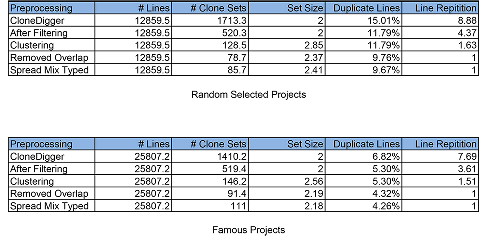
\epsfig{file=result1.pdf}
\caption{Preprocessing Results}
\end{figure}

\begin{figure}
\centering
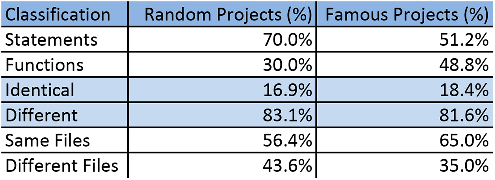
\epsfig{file=result3.pdf}
\caption{Classification Results}
\end{figure}

\begin{figure}
\centering
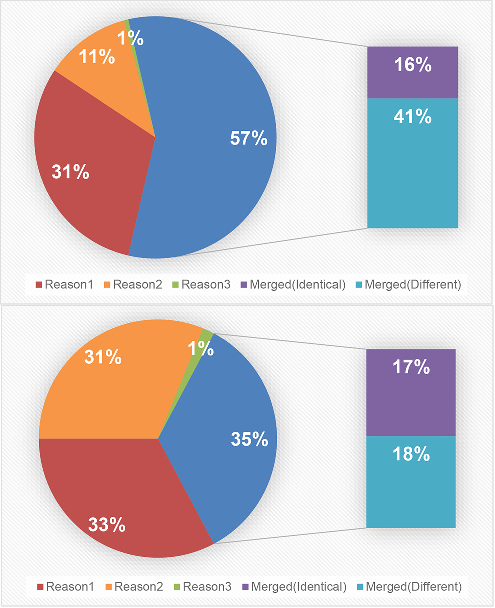
\epsfig{file=result2.pdf}
\caption{Mergeability Analysis}
\end{figure}

\begin{figure}
\centering
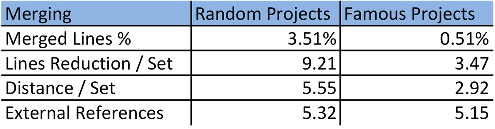
\epsfig{file=result4.pdf}
\caption{Merging Results}
\end{figure}

\begin{figure}
\centering
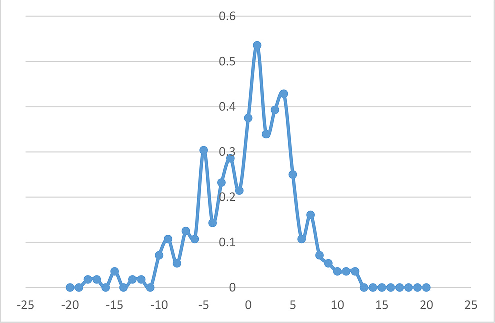
\epsfig{file=result5.pdf}
\caption{Recommendation Evaluation Distribution}
\end{figure}


\subsection{Preprocessing Results}
This test data in {\bf Figure 2.} shows number of lines, clone sets, set size, duplicate lines (lines in clone sets / total number of lines), and repeated lines for
both test sets after each filtering steps. As shown in the table, we removed many double counted clones. After all preprocessing steps, we have 9.67\% and
4.26\% duplicate lines left that we are able to merge, respectively, which is more than half of the code clones provided by CloneDigger. Set size was 2 before clustering
as set were pairs before the clustering step.

\subsection{Classification}
Classification test data in {\bf Figure 3.} shows how we classify clones into different types to handle them accordingly.
Statements and Functions data is very volatile as it somewhat depends on developers personal coding style.
Identical and Different data shows majority of clones we are merging are not Type-1, which correlates to our prediction
before the experiments as developers hardly actually copy and paste exact code. Same Files and Different Files shows that
it's slightly more common to have clone code residing in the same files, although we couldn't really reason about this observation.

\subsection{Mergeability Analysis}
{\bf Figure 4.} shows what percentage of code clones we can merge out of the ones provided by CloneDigger, and the distribution of clones 
we cannot handle according to different reasons:
\begin{itemize}
\item Reason 1: Type-3 clones - we are unable to merge any Type-3 clones at this moment
\item Reason 2: Clone Fragments of length which is too short. We don't want to merge these clones as it's not improving readability at all
\item Reason 3: Merges that throw unexpected exceptions for some reason that cannot pass our sanity check
\end{itemize}
We can merge almost all Type-1 clones and more than half of Type-2 clones. For clones that we cannot merge, most of them are Type-3 clones.

\subsection{Merging Results}
{\bf Figure 5.} shows the overall merging results. The data for random selected projects is more interesting as it is more practical for our
everyday software projects. The data is for merging all mergeable clones without considering any recommendation information. 
We can merge about 3.51\% code in total which is not a bad result, but each individual merge will only remove 9.21 lines of code in average
which is not very ideal but reasonable as it includes many not recommended merges of smaller line counts. Distance and external references
results tell that it's very common to have Type-2 clones and externality in code fragments. Note that external references value here include both
variable/function/objects references and returned variables for future reference. It shows we are rarely able to perform simple merges and need
to fix reference errors here and there.

\subsection{Recommendation Evaluation}
{\bf Figure 6.} is the distribution graph of our recommendation evaluation formula $f(RE)$. As we can see from the graph, about 45\% clones
are categorized as somewhat recommended to merge, while 40\% are not recommended with a below zero evaluation. And only around 15\% clones
are recommended. Which makes sense to us as we are only confident enough to merge clones that saves a lot of lines and do not introduce too much
extra complexity, and which only occupy a relatively small portion of all clones detected by CloneDigger. And we do want developers to actually
think about and make the merging decision carefully.

\subsection{Random Selected VS Famous Projects}
When comparing the results for our random selected projects and most famous projects from GitHub, the difference is quite noticeable.
Firstly, there are way less (almost half) duplicate lines in famous projects. Secondly, famous projects also have less set size which corresponds to
duplicate code across multiple fragments. Thirdly, for famous projects, most clone sets consist fragments inside same files, which means it has less 
``copy and paste" from file to file. Additionally, for all clone types detected in famous project, there are more Type-3 clones. In another word,
there are no simple clones for such famous projects, all occurrences of clones contain quite a few changes and semantics difference.
Lastly, based on more occurrence of Reason 2 unmergeable clones and lines reduction per set, clones in famous project are way smaller thus
less are actually clones which are meaningful to merge. The comparison result confirms our prediction that famous open source project are written
with better care and better refactored compared to random selected projects as they are backed by more professional developers and maintained by
bigger communities. We do not have access to any medium to large scale commercial propriety software project but we could assume they should
contain more clones and a higher percentage of those clones shall be merged as for such products delivery time may be more important than
code quality.

\subsection{Performance}
Performance-wise, as everything in our program works under O(n) time complexity, time to perform any kind of actions in EasyMerge is insignificant 
compared to CloneDigger which uses an algorithm of higher order. In fact, user will experience no delay whatsoever after the preprocessing step involving
CloneDigger is complete.


\section{Conclusion and Future Work}
Code clones are very common in medium to large scale software applications.
Detecting and refactoring unnecessary clones can help us provide cleaner, easier to understand, and readily reusable code.
However, there are many different types of clones and many subtle implications while dealing with them when coupling and
inheritance is involved. Our proposed solution, EasyMerge, is a clone refactoring tool based on anti-unification clone detector 
CloneDigger, that can handle most Type-1 clones and many Type-2 clones. It fixes external variable and function reference
and provide merge recommendation based on evaluation of externality and package information analysis.
Moreover, EasyMerge guarantees the consistency of functionality before and after code merging.

However, EasyMerge still has limitations. First of all, not all code clones can be detected by CloneDigger or any existing
code clone detection approach in general. For future work, we may upgrade EasyMerge's clone detection engine to locate
more clones in code base. Secondly, we can add support to merge more Type-2 and Type-3 clones (there is no reliable detection of Type-4 clones at the moment yet).
It's very challenging to merge Type-3 clones as we may need to add context-based analysis to sort out extra statements and different layouts of similar code.

Furthermore, the current version of EasyMerge cannot merge similar classes and all duplicated classes are filtered out in preprocessing.
In the future, we can add mechanism to merge similar classes, automatically generate parent classes and extract similar members and methods to the parents.
Additionally, current mergeable clones are within code blocks (at the same indentation level for Python). We are also interested in merging code clones that cross
multiple levels and scopes. We may break big clone fragments into smaller pieces and merge accordingly.
At the end, we couldn't implement mechanism in this version to detect intentionally introduced clones such as ones in test suites, which could 
also be a very good research direction for future work.


%ACKNOWLEDGMENTS are optional
%\section{Acknowledgements}

%
% The following two commands are all you need in the
% initial runs of your .tex file to
% produce the bibliography for the citations in your paper.
\bibliographystyle{abbrv}
\bibliography{paper}  % sigproc.bib is the name of the Bibliography in this case
% You must have a proper ".bib" file
%  and remember to run:
% latex bibtex latex latex
% to resolve all references
%
% ACM needs 'a single self-contained file'!
%
%APPENDICES are optional
%\balancecolumns
%\appendix
%Appendix A
%\subsection{References}
%Generated by bibtex from your ~.bib file.  Run latex,
%then bibtex, then latex twice (to resolve references)
%to create the ~.bbl file.  Insert that ~.bbl file into
%the .tex source file and comment out
%the command \texttt{{\char'134}thebibliography}.
%\balancecolumns
% That's all folks!
\end{document}
